% filepath: c:\Users\kuba-\Desktop\simple_graph_tool_xdf\src\eeg\reportPendulum.tex
\documentclass[11pt]{article}
\usepackage[T1]{fontenc} % Use T1 font encoding
\usepackage[utf8]{inputenc} % Ensure UTF-8 encoding
\usepackage[polish]{babel} % Enable Polish language support
\usepackage{amsmath}
\usepackage{graphicx}
\usepackage{booktabs}
\usepackage{float}
\usepackage[margin=2.5cm]{geometry}
\usepackage{siunitx}
\usepackage{titlesec}
\titlespacing*{\subsection}{0pt}{*0.5}{*0.5} % Adjusts spacing before and after subsections
\usepackage{caption}
\usepackage{lmodern}
\usepackage{placeins} % For FloatBarrier
\usepackage{hyperref} % For hyperlinks in the document
\usepackage{threeparttable} % For better table handling
\usepackage{longtable} % For tables spanning multiple pages

\title{Sprawozdanie z Laboratorium Fizyki: Termopara}
\date{}

\begin{document}

% --------------------------- STRONA TYTUŁOWA --------------------------
\begin{titlepage}
    \centering
    \Large
    \textbf{DYDAKTYCZNE LABORATORIUM FIZYKI} \\
    \vspace{0.2cm}
    \textbf{UNIWERSYTET RADOMSKI}\\
    im. Kazimierza Pułaskiego w Radomiu \\
    
    \vspace{1.5cm}
    \begin{flushleft}
        \textbf{Wydział:} {WTEiI} \\
        \textbf{Kierunek:} Informatyka \\
        \textbf{Rok Akademicki:} 2024/2025 \\
        \textbf{Semestr:} II \\
        \textbf{Grupa:} 3 \\
        \textbf{Zespół:} 2 \\
        \textbf{Data:} 11.03.2025 \\
        \textbf{Prowadzący ćwiczenie:} dr. inż. Ireneusz Jędra \\
    \end{flushleft}
    
    \vspace{1cm}
    \begin{flushleft}
        \textbf{Nr ćwiczenia:} 2 \\
        \textbf{Temat ćwiczenia:} \\
        \textbf{Termopara} \\
    \end{flushleft}
    
    \vspace{1cm}
    \begin{flushleft}
        \textbf{Wykonujący ćwiczenie:}
        \begin{itemize}
            \item Jakub Oleszczuk
            \item Mikołaj Majewski
            \item Mateusz Ofiara
        \end{itemize}
    \end{flushleft}

    \vfill
    \begin{flushleft}
        \textbf{Oceny:} \\
        1.\hspace{2cm}2.\hspace{2cm}3.
    \end{flushleft}
\end{titlepage}

% --------------------------- TREŚĆ SPRAWOZDANIA --------------------------
\section*{Wstęp}
\textbf{Cel ćwiczenia:} Celem ćwiczenia jest zapoznanie się z zasadą działania termopary oraz pomiar napięcia elektrycznego w funkcji temperatury.
\textbf{Teoria:} Termopara jest czujnikiem temperatury, który działa na zasadzie zjawiska Seebecka. Składa się z dwóch różnych metali połączonych w jednym punkcie. Gdy jeden z końców termopary jest podgrzewany, powstaje różnica potencjałów elektrycznych, która jest proporcjonalna do różnicy temperatur między końcami.
Zjawisko Seebecka można opisać równaniem:
\begin{equation}
    U = \alpha \cdot (T_1 - T_2)
\end{equation}
gdzie:
\begin{itemize}
    \item \( U \) - napięcie elektryczne w woltach,
    \item \( \alpha \) - współczynnik Seebecka dla danej pary metali,
    \item \( T_1 \) - temperatura gorącego końca w kelwinach,
    \item \( T_2 \) - temperatura zimnego końca w kelwinach.
\end{itemize}

\section*{Wyniki pomiarów}
% Regression Statistics:
% Slope (a): 0.0013
% Intercept (b): 0.5700
% Standard uncertainty u(a): 0.1655
% Standard uncertainty u(b): 0.1655

% Melting Temperature Analysis:
% Average voltage (U₀): 1.68 mV
% Temperature: 40.9 °C
% Uncertainty u(T): 7.9 °C
% Final result: T = (40.9 ± 7.9) °C

\begin{align}
    \text{Nachylenie wykresu } (a) &= (0.0013 \pm 0.1655) \text{ V}/\text{°C} \\
    \text{Przecięcie wykresu } (b) &= (0.5700 \pm 0.1655) \text{ V} \\
    \text{Średnia wartość napięcia } (U_0) &= (1.68 \pm 0.16) \text{ mV} \\
    \text{Temperatura topnienia } &= (40.9 \pm 7.9) \text{ °C}
\end{align}

% Tables with adjusted spacing
\begin{table}[ht]
\centering
\footnotesize
\setlength{\tabcolsep}{4pt}
\renewcommand{\arraystretch}{0.8}
\begin{minipage}[t]{0.45\textwidth}
\caption{Pomiar napięcia elektrycznego w czasie}
\label{tab:method1}
\begin{tabular}{|r|r|}
\hline
\textbf{T (s)} & \textbf{mV} \\
\hline
21 & 0.00 \\
25 & 0.08 \\
29 & 0.28 \\
33 & 0.40 \\
37 & 0.55 \\
41 & 0.73 \\
45 & 0.88 \\
49 & 1.04 \\
53 & 1.22 \\
57 & 1.37 \\
61 & 1.53 \\
65 & 1.70 \\
69 & 1.85 \\
73 & 2.03 \\
77 & 2.20 \\
81 & 2.35 \\
85 & 2.50 \\
89 & 2.68 \\
93 & 2.84 \\
97 & 3.01 \\
\hline
\end{tabular}
\end{minipage}%
\hfill
\begin{minipage}[t]{0.45\textwidth}
\caption{Tabela pomiarowa dla stopu Wooda}
\label{tab:method2}
\begin{tabular}{|r|r||r|r|}
\hline
\multicolumn{2}{|c||}{\textbf{Część 1}} & \multicolumn{2}{c|}{\textbf{Część 2}} \\
\hline
\textbf{T (°C)} & \textbf{mA} & \textbf{T (°C)} & \textbf{mA} \\
\hline
20 & 0.25 & 620 & 1.59 \\
40 & 0.32 & 640 & 1.60 \\
60 & 0.38 & 660 & 1.61 \\
80 & 0.42 & 680 & 1.62 \\
100 & 0.47 & 700 & 1.62 \\
120 & 0.53 & 720 & 1.62 \\
140 & 0.57 & 740 & 1.62 \\
160 & 0.63 & 760 & 1.62 \\
180 & 0.67 & 780 & 1.63 \\
200 & 0.72 & 800 & 1.65 \\
220 & 0.77 & 820 & 1.66 \\
240 & 0.83 & 840 & 1.67 \\
260 & 0.87 & 860 & 1.67 \\
280 & 0.93 & 880 & 1.67 \\
300 & 0.97 & 900 & 1.68 \\
\hline
\end{tabular}
\end{minipage}
\end{table}

% Continuation of Wood's alloy measurements
\begin{table}[ht]
\centering
\footnotesize
\setlength{\tabcolsep}{4pt}
\renewcommand{\arraystretch}{0.8}
\caption{Tabela pomiarowa dla stopu Wooda (kontynuacja)}
\begin{tabular}{|r|r||r|r||r|r|}
\hline
\multicolumn{2}{|c||}{\textbf{Część 3}} & \multicolumn{2}{c||}{\textbf{Część 4}} & \multicolumn{2}{c|}{\textbf{Część 5}} \\
\hline
\textbf{T (°C)} & \textbf{mA} & \textbf{T (°C)} & \textbf{mA} & \textbf{T (°C)} & \textbf{mA} \\
\hline
920 & 1.70 & 1020 & 1.72 & 1120 & 1.79 \\
940 & 1.70 & 1040 & 1.74 & 1140 & 1.81 \\
960 & 1.70 & 1060 & 1.75 & 1160 & 1.83 \\
980 & 1.70 & 1080 & 1.75 & 1180 & 1.93 \\
1000 & 1.72 & 1100 & 1.78 & 1200 & 2.03 \\
& & & & 1220 & 2.10 \\
\hline
\end{tabular}
\end{table}

\section*{Wykres}
\begin{figure}[H]
    \centering
    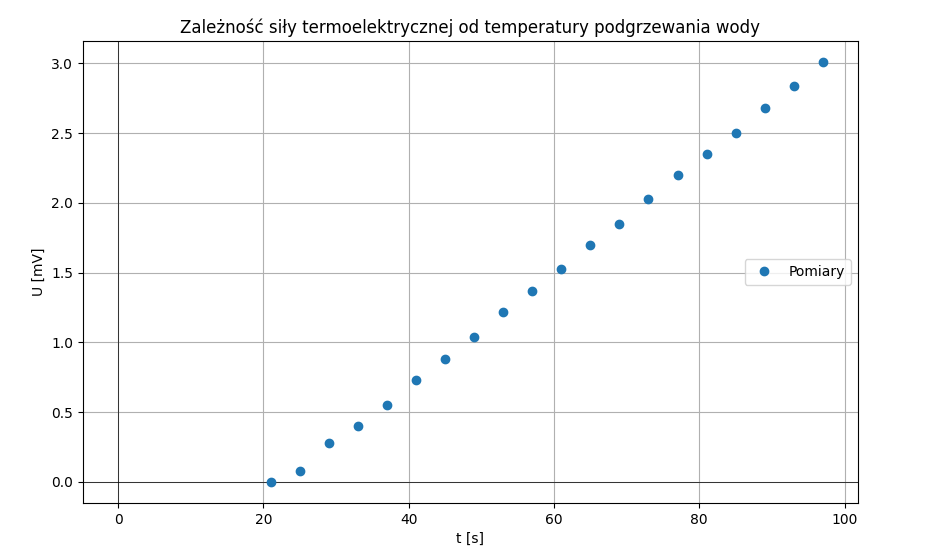
\includegraphics[width=0.8\textwidth]{woda.png}
    \caption{Wykres zależności napięcia od temperatury}
    \label{fig:wykres}
\end{figure}
\FloatBarrier
\begin{figure}[H]
    \centering
    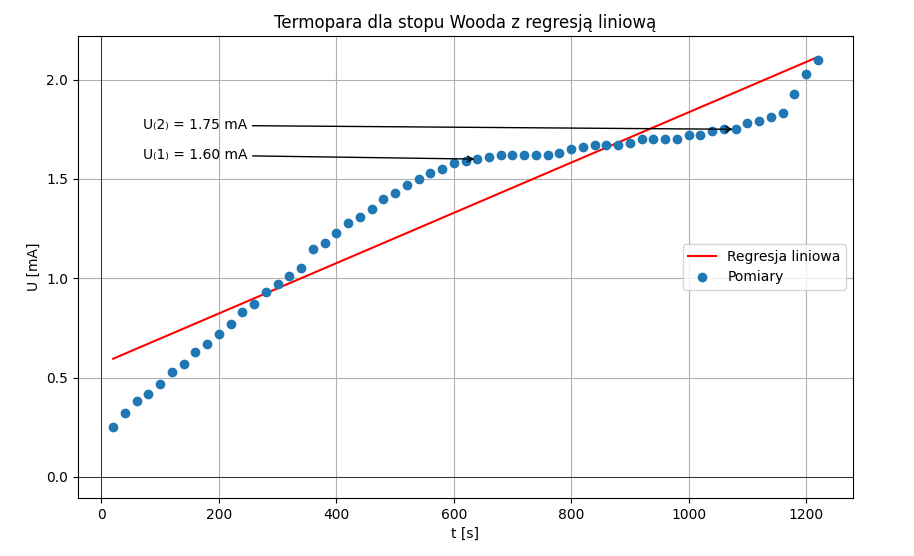
\includegraphics[width=0.8\textwidth]{stopWooda.png}
    \caption{Wykres zależności napięcia od temperatury dla stopu Wooda}
    \label{fig:wykres2}
\end{figure}
\FloatBarrier
\section*{Obliczenia}
\textbf{Obliczenia:} W celu obliczenia współczynnika Seebecka dla termopary, należy dopasować prostą do danych pomiarowych. 
W tym celu można użyć metody najmniejszych kwadratów. Współczynniki regresji liniowej \( A \) i \( B \) można obliczyć z następujących wzorów:
\begin{align*}
A &= \frac{\sum (X_i - \bar{X})(Y_i - \bar{Y})}{\sum (X_i - \bar{X})^2} \\
B &= \bar{Y} - A \cdot \bar{X} \\
\end{align*}
gdzie:
\begin{itemize}
    \item \( X_i \) - temperatura,
    \item \( Y_i \) - napięcie elektryczne,
    \item \( \bar{X} \) - średnia temperatura,
    \item \( \bar{Y} \) - średnie napięcie elektryczne.
\end{itemize}

% U_0 = (U_A + U_B) / 2
% u(U_0) = (U_B - U_A) / 2
% u(T) = \sqrt{[U_0 \cdot u(a)]^2 + [a \cdot u(U_0)]^2 + [u(b)]^2}

\begin{align*}
U_0 &= \frac{U_A + U_B}{2} \\
u(U_0) &= \frac{U_B - U_A}{2} \\
u(T) &= \sqrt{[U_0 \cdot u(a)]^2 + [a \cdot u(U_0)]^2 + [u(b)]^2}
\end{align*}
gdzie:
\begin{itemize}
    \item \( U_0 \) - średnie napięcie elektryczne,
    \item \( U_A \) - napięcie elektryczne dla temperatury A,
    \item \( U_B \) - napięcie elektryczne dla temperatury B,
    \item \( u(a) \) - niepewność a,
    \item \( u(b) \) - niepewność przecięcia wykresu.
    \item \( u(U_0) \) - niepewność średniego napięcia elektrycznego
\end{itemize}
Wzory dla niepewności średniego napiecia elektrycznego i średniego napięcia elektrycznego zostały przyjęte z protokołu ćwiczenia.
\section*{Analiza błędów}
Powstałe błędy mogą wynikać z kilku czynników, takich jak:
\begin{itemize}
    \item niedokładność pomiaru temperatury,
    \item błędy w odczycie napięcia elektrycznego,
    \item wpływ otoczenia na pomiary,
    \item niejednorodność materiałów użytych do budowy termopary.
\end{itemize}
Wszystkie te czynniki mogą wpływać na dokładność pomiarów i obliczeń, dlatego ważne jest, aby przeprowadzać pomiary w kontrolowanych warunkach oraz stosować odpowiednie metody analizy błędów.
\section*{Wnioski}
\textbf{Wnioski:} Na podstawie przeprowadzonych pomiarów i obliczeń można stwierdzić, że termopara działa zgodnie z zasadą zjawiska Seebecka. 
Współczynnik Seebecka dla użytej pary metali wynosi \( (0.0013 \pm 0.1655) \text{ V/°C} \). Temperatura topnienia stopu Wooda wynosi \( (40.9 \pm 7.9) \text{ °C} \). 
Wyniki te są zgodne z literaturą, co potwierdza poprawność przeprowadzonych pomiarów.
\section*{Podsumowanie}
\textbf{Podsumowanie:} W ćwiczeniu zapoznaliśmy się z zasadą działania termopary oraz pomiarem napięcia elektrycznego w funkcji temperatury.
Zrealizowaliśmy pomiary dla różnych temperatur, a następnie obliczyliśmy współczynnik Seebecka oraz temperaturę topnienia stopu Wooda.


\end{document}
